Applications develop for mobile platforms can be tricky to test.
It exists simulations, but this does not guarantee that the model will be applicable in practice.
Standard emulators are limited by their lack of support for WiFi-Direct and large-scale deployment.
In this section, we present our own large-scale emulation platform called AndroFleet that provides us a good testing tool for our approach.

Pourquoi wi-fi direct simulation ??? (pas de base dans android emulator)


When comes the evaluation time, three way offer to us.
- real devices
- simulators
- emulators

A lot of proposition are simulation platform instead of emulation platform.
Simulation platform are the way when we need performance and rapidity in testing.
Emulation platform are more to test as near as possible an application in a real case.


Simulation platform permit to test an approach faster than emulation platform because 

First, we have the simulator tool family.
Simulators aim to reproduct a the basic--or a substract--behaviour of a system.

The simulators aims to findely reproduct a behaviour.
For instance, a WiFi simulator can reproduct with a high fidelity the WiFi signal behaviour like signal degradation in function of the environment.

The second, we have the emulator tool family.
Emulators aim to exactly replicate the behaviour of a system.
An emulator is a complete replication of the system emulated.
The emulators are closer to the system than simulators.

Why emulation over simulation ?

Because it does not exist emulators that match or can be adapted to our requirements, we develop AndroFleet, our large-scale emulation platform.

We want an emulation platform instead of simulation because we want to test our approach as near as possible of a real case.

We want to be able to reproduce scenarii to be able to compare different approaches.


reproducibility of the experiment with random seed.

% Why AndroFleet ???

For example, none of Android or iOS emulators support proximity wireless interactions and the only
way is to test them is to use real devices.
However, this method does not scale and cannot reproduce realistic events that can be encountered in real deployments. 
Another limitation in the geo-privacy field is the incapacity to reproduce and compare experiments. Geo-privacy focuses its interest on the critical impact of location data on users privacy. 
In this domains, the evaluation builds on shared datasets, which are used by the community to test and assess their algorithms. 
However, these datasets are often altered for the purpose of evaluation and this modification of the input data prevents from further comparisons.
Finally, in the mobile computing community, some simulation tools give the opportunity to simulate many devices, network and others. 
However, these tools are not focused on crowd-sensing concerns like wireless proximity issues or the validation on a very large number of emulators running and moving at the same time.

%%%% OK

\subsection{Overview of AndroFleet}

AndroFleet is a large-scale emulation platform that allows to test our Android library.
The platform deploys and runs a large amount of emulators at the same time on a single or multiple hosts.
AndroFleet allows to run GPS location scenarios that reproduced real users' movements.
Lastly, the platform includes a Wi-Fi Direct simulator that allows the use of the Wi-Fi Direct in the Android emulators.

We choose to use the Docker technology because it allows to package and deploy containers easily on different hosts.
Moreover, this technology allows to reproduce behaviours because each time a container is launched, a clean instance of the system is set.
Finally, we use Weave, a technology working with Docker, which manages the containers' network.

\begin{figure*}[h]
	\centering
	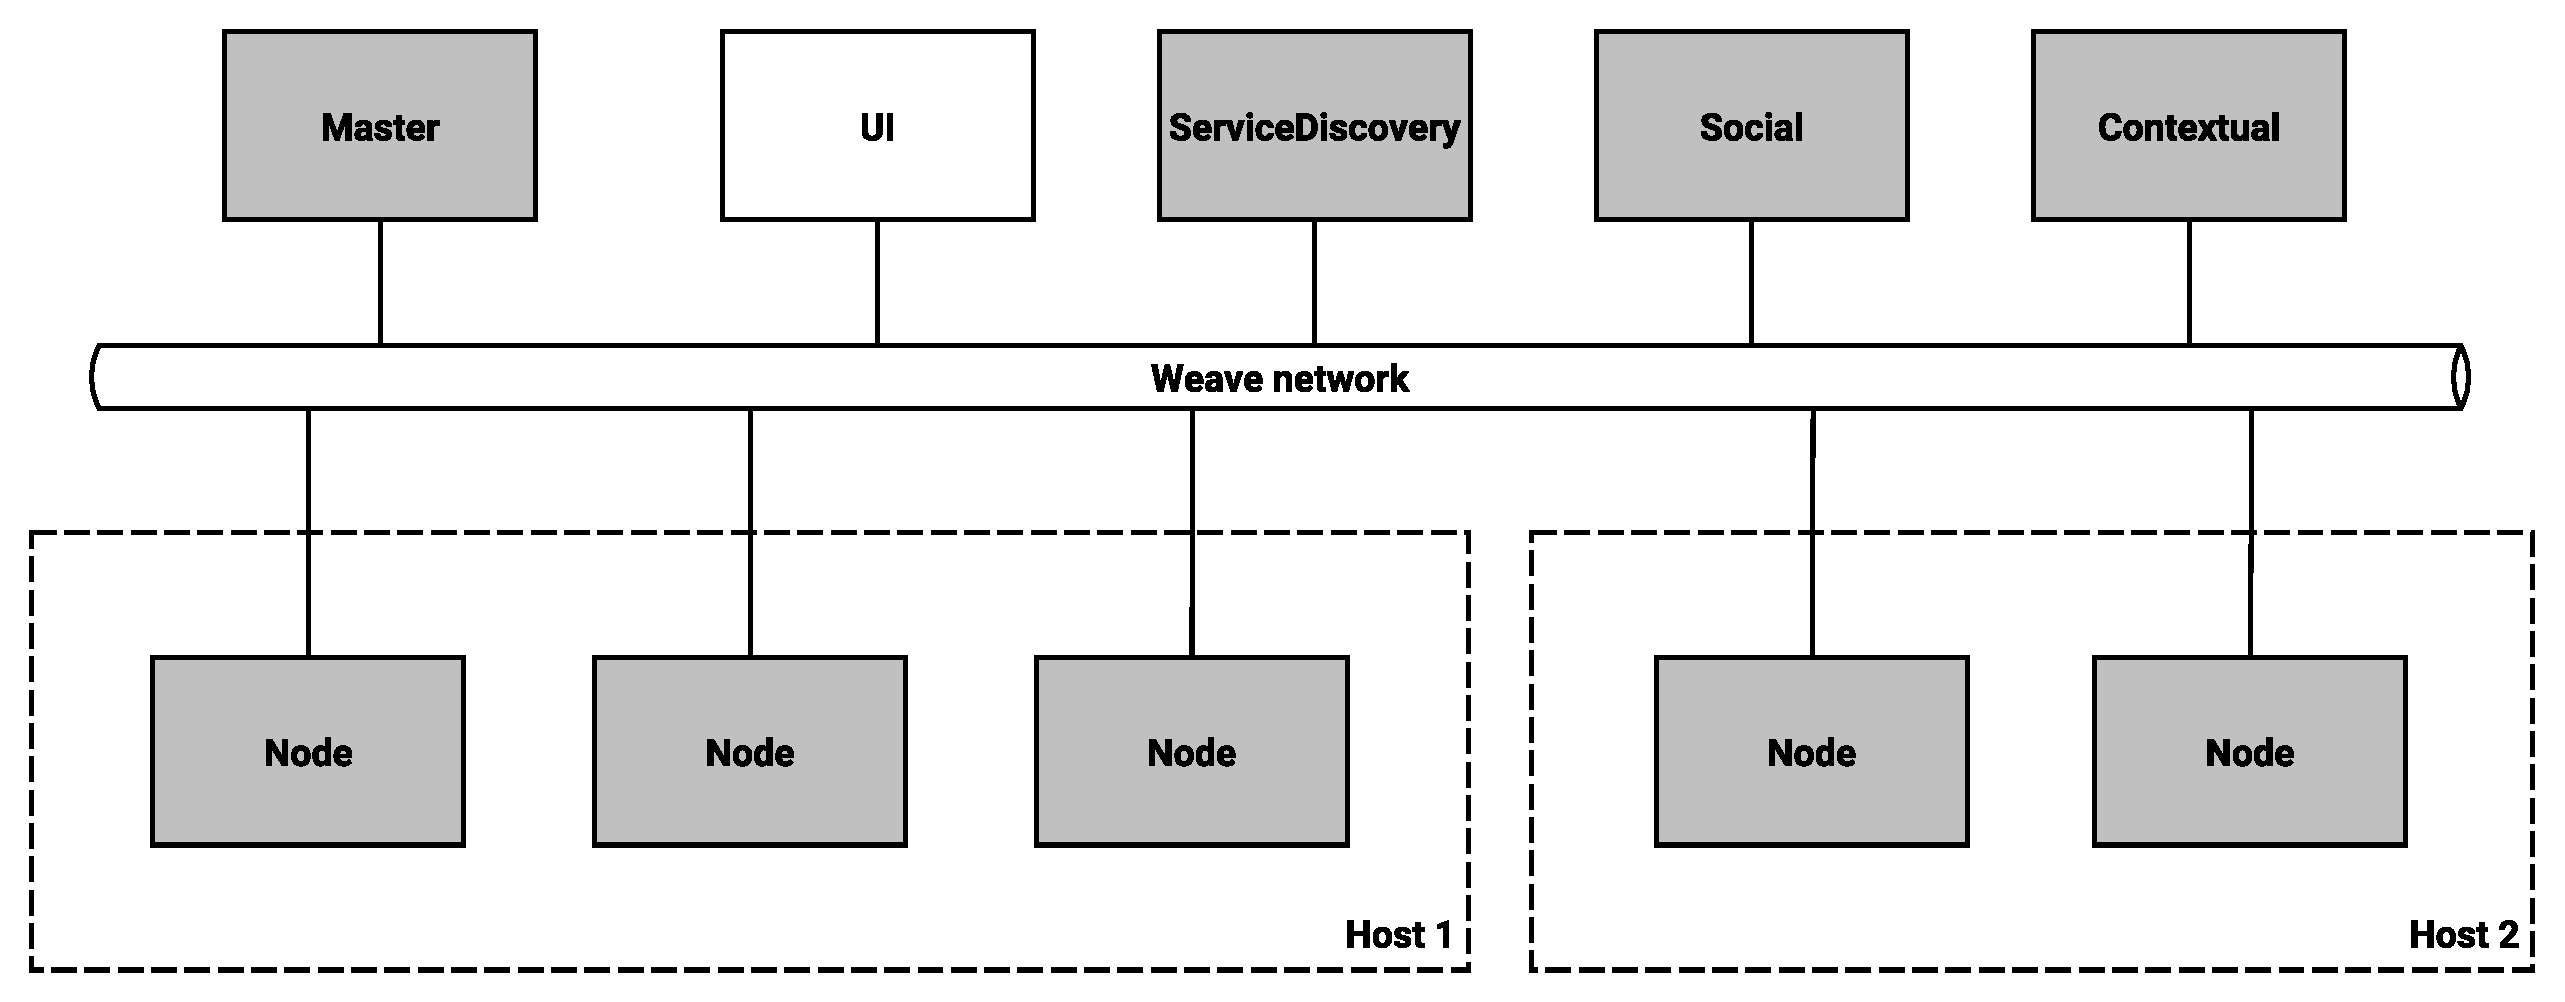
\includegraphics[width=\textwidth]{figures/androfleet}
	\caption{\label{AndroFleet} AndroFleet architecture}
\end{figure*}

The architecture of AndroFleet, presented in the Figure~\ref{AndroFleet}, is composed of 5 elements: Master, Node, ServiceDiscovery, Social, Contextual and UI.
All these elements are packaged and regrouped in a single Docker container.
This container includes an Android emulator that will be run by the Node.

The Master is the main element of the architecture.
It communicates with all other elements of the platform.
For instance, this element is responsible to attribute a scenario to each node container connected.
The Master synchronizes elements of the system.
It allows to control emulation steps with a Command Line Interface and provides information about the progress of the emulation.

The Node element is responsible to launch the Android emulator included in the container and play a GPS scenario.

The ServiceDiscovery element is used for the Wi-Fi Direct simulator.
It allows to the devices to discover themselves.
A Node can request it a list of all its neighbors given its current GPS position.

The Social elements contain information of existing links that exist between emulated users.
The element generates for each running Node its social links.

The Contextual element has the same behaviour as the Social one.
This element generates contextual information for each Node.

The UI is an optional part that can be used to visualize the GPS position of each Android emulator on a map.

A GeoLife parser is included and it permits to recreate files that are used in our experiment.

\subsection{Evaluation Protocol}

%%%% END OK

First
Then, we evaluate the scenarii runner on the well known GeoLife dataset.
We choose Geolife because it is the reference database used by researchers in the geo-location privacy research.
Geolife is a GPS trajectory dataset collected by 178 different users in a period of over 4 years. 
This dataset contains a total of 17,621 trajectories.

Each trace is timestamped.

We process the traces and see if WiFi-Direct can appear with these.

Geolife dataset
We run experiments using the Microsoft’s Geolife
dataset that is a GPS trajectory dataset.
This dataset is made of 182 users for a period of over three years.
In this dataset, a GPS trajectory is represented by a
sequence of time-stamped points.
Each points contains a latitude, longitude and altitude value.
The distance cover by the dataset is about 1.2 million kilometers.
The total duration of timestamp traces is about 48.000 hours.
About 90\% of data logged are spaced under 5 seconds.


so we process Geolife data to regroup traces 

\subsection{Evaluation Results}